% Soubory musí být v kódování, které je nastaveno v příkazu \usepackage[...]{inputenc}

\documentclass[%        Základní nastavení
  %draft,    				  % Testovací překlad
  12pt,       				% Velikost základního písma je 12 bodů
	t,                  % obsah slajdů bude vždy začínat od shora (nebude vertikálně centrovaný)
	aspectratio=1610,   % poměr stran bude 16:10 (všechny projektory v učebnách na Technické 12 Brno),
	                    % další volby jsou 43, 149, 169, 54, 32.
	unicode,						% Záložky a informace budou v kódování unicode
]{beamer}				    	% Dokument třídy 'zpráva', vhodná pro sazbu závěrečných prací s kapitolami
%\usepackage{etex}

\usepackage[utf8]		  % Kódování zdrojových souborů je v UTF-8
	{inputenc}					% Balíček pro nastavení kódování zdrojových souborů
	
\usepackage{graphicx} % Balíček 'graphicx' pro vkládání obrázků
											% Nutné pro vložení logotypů školy a fakulty

\usepackage[          % Balíček 'acronym' pro sazby zkratek a symbolů
	nohyperlinks				% Nebudou tvořeny hypertextové odkazy do seznamu zkratek
]{acronym}						
											% Nutné pro použití prostředí 'acronym' balíčku 'thesis'

%% Balíček hyperref je volán třídou beamer automaticky, proto není třeba následujícího kódu:
%\usepackage[
%	breaklinks=true,		% Hypertextové odkazy mohou obsahovat zalomení řádku
%	hypertexnames=false % Názvy hypertextových odkazů budou tvořeny
%											% nezávisle na názvech TeXu
%]{hyperref}						% Balíček 'hyperref' pro sazbu hypertextových odkazů
%											% Nutné pro použití příkazu 'nastavenipdf' balíčku 'thesis'

\usepackage{cmap} 		% Balíček cmap zajišťuje, že PDF vytvořené `pdflatexem' je
											% plně "prohledávatelné" a "kopírovatelné"

%\usepackage{upgreek}	% Balíček pro sazbu stojatých řeckých písmem
											%% např. stojaté pí: \uppi
											%% např. stojaté mí: \upmu (použitelné třeba v mikrometrech)
											%% pozor, grafická nekompatibilita s fonty typu Computer Modern!

%\usepackage{amsmath} %balíček pro sabu náročnější matematiky

\usepackage{booktabs} % Balíček, který umožňuje v tabulce používat
% příkazy \toprule, \midrule, \bottomrule









\usepackage[absolute,overlay]{textpos}





%%%%%%%%%%%%%%%%%%%%%%%%%%%%%%%%%%%%%%%%%%%%%%%%%%%%%%%%%%%%%%%%%
%%%%%%      Definice informací o dokumentu             %%%%%%%%%%
%%%%%%%%%%%%%%%%%%%%%%%%%%%%%%%%%%%%%%%%%%%%%%%%%%%%%%%%%%%%%%%%%

% V tomto souboru se nastavují téměř veškeré informace, proměnné mezi studenty:
% jméno, název práce, pohlaví atd.
% Tento soubor je SDÍLENÝ mezi textem práce a prezentací k obhajobě -- netřeba něco nastavovat na dvou místech.

\usepackage[
%%% Z následujících voleb jazyka lze použít pouze jednu
  czech-english,		% originální jazyk je čeština, překlad je anglicky (výchozí)
  %english-czech,	  % originální jazyk je angličtina, překlad je česky
  %slovak-english,	% originální jazyk je slovenština, překlad je anglicky
  %english-slovak,	% originální jazyk je angličtina, překlad je slovensky
%
%%% Z následujících voleb typu práce lze použít pouze jednu
  %semestral,		  % semestrální práce (výchozí)
  bachelor,			%	bakalářská práce
  %master,			  % diplomová práce
  %treatise,			% pojednání o disertační práci
  %doctoral,			% disertační práce
%
%%% Z následujících voleb zarovnání objektů lze použít pouze jednu
%  left,				  % rovnice a popisky plovoucích objektů budou zarovnány vlevo
	center,			    % rovnice a popisky plovoucích objektů budou zarovnány na střed (vychozi)
%
]{thesis}   % Balíček pro sazbu studentských prací


%%% Jméno a příjmení autora ve tvaru
%  [tituly před jménem]{Křestní}{Příjmení}[tituly za jménem]
% Pokud osoba nemá titul před/za jménem, smažte celý řetězec '[...]'
\author[]{Tomáš}{Vavrinec}

%%% Identifikační číslo autora (VUT ID)
\butid{240893}

%%% Pohlaví autora/autorky
% (nepoužije se ve variantě english-czech ani english-slovak)
% Číselná hodnota: 1...žena, 0...muž
\gender{0}

%%% Jméno a příjmení vedoucího/školitele včetně titulů
%  [tituly před jménem]{Křestní}{Příjmení}[tituly za jménem]
% Pokud osoba nemá titul před/za jménem, smažte celý řetězec '[...]'
\advisor[doc.\ Ing..]{Pavel}{Šteffan}[Ph.D.]

%%% Jméno a příjmení oponenta včetně titulů
%  [tituly před jménem]{Křestní}{Příjmení}[tituly za jménem]
% Pokud osoba nemá titul před/za jménem, smažte celý řetězec '[...]'
% Nastavení oponenta se uplatní pouze v prezentaci k obhajobě;
% v případě, že nechcete, aby se na titulním snímku prezentace zobrazoval oponent, pouze příkaz zakomentujte;
% u obhajoby semestrální práce se oponent nezobrazuje (jelikož neexistuje)
% U dizertační práce jsou typicky dva až tři oponenti. Pokud je chcete mít na titulním slajdu, prosím ručně odkomentujte a upravte jejich jména v definici "VUT title page" v souboru thesis.sty.
\opponent[doc.\ Ing.]{Jiří }{Háze}[Ph.D.]

%%% Název práce
%  Parametr ve složených závorkách {} je název v originálním jazyce,
%  parametr v hranatých závorkách [] je překlad (podle toho jaký je originální jazyk).
%  V případě, že název Vaší práce je dlouhý a nevleze se celý do zápatí prezentace, použijte příkaz
%  \def\insertshorttitle{Zkác.\ náz.\ práce}
%  kde jako parametr vyplníte zkrácený název. Pokud nechcete zkracovat název, budete muset předefinovat,
%  jak se vytváří patička slidu. Viz odkaz: https://bit.ly/3EJTp5A
\title[Title of Student's Thesis]{Automatické herní stanoviště}

%%% Označení oboru studia
%  Parametr ve složených závorkách {} je název oboru v originálním jazyce,
%  parametr v hranatých závorkách [] je překlad
\specialization[Microelectronics and Technology]{Mikroelektronika a technologie}

%%% Označení ústavu
%  Parametr ve složených závorkách {} je název ústavu v originálním jazyce,
%  parametr v hranatých závorkách [] je překlad
%\department[Department of Control and Instrumentation]{Ústav automatizace a měřicí techniky}
%\department[Department of Biomedical Engineering]{Ústav biomedicínského inženýrství}
%\department[Department of Electrical Power Engineering]{Ústav elektroenergetiky}
%\department[Department of Electrical and Electronic Technology]{Ústav elektrotechnologie}
%\department[Department of Physics]{Ústav fyziky}
%\department[Department of Foreign Languages]{Ústav jazyků}
%\department[Department of Mathematics]{Ústav matematiky}
\department[Department of Microelectronics]{Ústav mikroelektroniky}
%\department[Department of Radio Electronics]{Ústav radioelektroniky}
%\department[Department of Theoretical and Experimental Electrical Engineering]{Ústav teoretické a experimentální elektrotechniky}
% \department[Department of Telecommunications]{Ústav telekomunikací}
%\department[Department of Power Electrical and Electronic Engineering]{Ústav výkonové elektrotechniky a elektroniky}

%%% Označení fakulty
%  Parametr ve složených závorkách {} je název fakulty v originálním jazyce,
%  parametr v hranatých závorkách [] je překlad
%\faculty[Faculty of Architecture]{Fakulta architektury}
\faculty[Faculty of Electrical Engineering and~Communication]{Fakulta elektrotechniky a~komunikačních technologií}
%\faculty[Faculty of Chemistry]{Fakulta chemická}
%\faculty[Faculty of Information Technology]{Fakulta informačních technologií}
%\faculty[Faculty of Business and Management]{Fakulta podnikatelská}
%\faculty[Faculty of Civil Engineering]{Fakulta stavební}
%\faculty[Faculty of Mechanical Engineering]{Fakulta strojního inženýrství}
%\faculty[Faculty of Fine Arts]{Fakulta výtvarných umění}
%
%Nastavení logotypu (v hranatych zavorkach zkracene logo, ve slozenych plne):
\facultylogo[logo/FEKT_zkratka_barevne_PANTONE_CZ]{logo/UTKO_color_PANTONE_CZ}

%%% Rok odevzdání práce
\graduateyear{2025}
%%% Akademický rok odevzdání práce
\academicyear{2024/25}

%%% Datum obhajoby (uplatní se pouze v prezentaci k obhajobě)
\date{17.\,6.\,2025} 

%%% Místo obhajoby
% Na titulních stránkách bude automaticky vysázeno VELKÝMI písmeny (pokud tyto stránky sází šablona)
\city{Brno}

%%% Abstrakt
\abstract[%
The goal of this thesis is to design and operate an electronic device for use in outdoor games. 
The primary goal, to create an automated game station, was extended to design a simple personal device as well. 
This thesis aims to design and to create a working electronic device with its own cover shell. 
It emphasizes the right choice of system solutions for the application in the outdoor games and the correct design of the electrical circuits. 
The thesis is divided into several parts - the introduction describes the requirements of the games, the design of a simple personal device and the design of a game with the primary goal of designing a core and evaluating game results. 
]{%
Cílem práce je navrhnout a~zprovoznit elektronické zařízení pro využití v outdoorových hrách. 
Primárně jde o~návrh automatického herního stanoviště, ale došlo i~k~návrhu jednoduchého osobního zařízení. 
Tato práce se zabývá návrhem a~následným oživením elektroniky a~navíc návrhem jejího krytu.
Je kladen důraz na výběr vhodných systémů k~aplikaci ve hrách a~z~nich vycházející návrh elektroniky.
Práce je rozdělena do několika skupin, uvod popisující požadavky her, návrh osobního zařízení a~návrh herního stanoviště, který se zabývá primárně návrhem jádra a~následné zhodnotecní výsledků.
}

%%% Klíčová slova
\keywrds[%
microcontroller, ESP32, ESP32-C3-MINI-1, ESP32-S3, ESP32-S3-WROOM, outdoor games, gaming stations, gaming facilities
]{%
mikrokontrolér, ESP32, ESP32-C3-MINI-1, ESP32-S3, ESP32-S3-WROOM, outdoorové hry, herní stanoviště, herní zařízení
% Klíčová slova v~originálním jazyce
}

%%% Poděkování
\acknowledgement{%
  Rád bych poděkoval vedoucímu bakalářské práce panu doc. Ing. Pavlu Šteffanovi, Ph.D.\ za konzultace, trpělivost a návrhy k~práci.
  Dále bych chtěl poděkovat svému švagrovi Ing. Janu Kirchnerovi za užitečné návrhy ke konstrukci krytů zařízení, k technoligii jejich výroby a především za umožnění využití jeho pětihlavé tiskárny.
  Také bych rád poděkoval mé matce Ing. Věře Vavrincové, přítelkyni Bc. Lucii Rebrovej a především kolegovi Mgr. Petru Kubicovi za kontrolu a připomínky k textové stránce práce.
  % Nakonec bych chtěl poděkovat jednomu nespolehlivému programátorovi Bc. Tomáši Rohlinkovi za to, že si zaplatil výroby prototypu a možná dodá kod na prezentaci práce.
  % Zvláštní poděkování patří Bc. Tomáši Rohlinkovi, který ochotně financoval výrobu prototypu AHS a~možná i~dodá kód k~przentaci práce.
}%
      % v tomto souboru doplňte údaje o sobě, o názvu práce...
                       % (tento soubor je sdílený s textem práce)

%%%%%%%%%%%%%%%%%%%%%%%%%%%%%%%%%%%%%%%%%%%%%%%%%%%%%%%%%%%%%%%%%%%%%%%%

%%%%%%%%%%%%%%%%%%%%%%%%%%%%%%%%%%%%%%%%%%%%%%%%%%%%%%%%%%%%%%%%%%%%%%%%
%%%%%%     Nastavení polí ve Vlastnostech dokumentu PDF      %%%%%%%%%%%
%%%%%%%%%%%%%%%%%%%%%%%%%%%%%%%%%%%%%%%%%%%%%%%%%%%%%%%%%%%%%%%%%%%%%%%%
%% Při vloženém balíčku 'hyperref' lze použít příkaz '\pdfsettings'
\pdfsettings
%  Nastavení polí je možné provést také ručně příkazem:
%\hypersetup{
%  pdftitle={Název studentské práce},    	% Pole 'Document Title'
%  pdfauthor={Autor studenstké práce},   	% Pole 'Author'
%  pdfsubject={Typ práce}, 						  	% Pole 'Subject'
%  pdfkeywords={Klíčová slova}           	% Pole 'Keywords'
%}
\hypersetup{pdfpagemode=FullScreen}       % otevření rovnou v režimu celé obrazovky
%%%%%%%%%%%%%%%%%%%%%%%%%%%%%%%%%%%%%%%%%%%%%%%%%%%%%%%%%%%%%%%%%%%%%%%

\usetheme{VUT} 				% barvy a rozložení prezentace odpovídající VUT FEKT
% alternativně lze použít jiná berevná témata, ale bez záruky. Například: 
%\usetheme{Darmstadt} \usecolortheme{default2}
\logoheader					% vytvoření zkráceného loga VUT FEKT v hlavičce slajdu, nechte odkomentované


\begin{document}

% v případě zakomentování následujícího se zobrazí v pravém dolním rohu slajdů klikatelné navigační symboly 
\disablenavigationsymbols

% titulní snímek, vysazen bez horních, dolních a postranních lišt (volba plain),
% není tak vysazen ani nadpis snímku
\maketitle

%%%%%%%%%%%%%%%%%%%%%%%%%%%%%%%%%%%%%%%%%%%%%%%%%%%%%%%%%%%%%%%%%%%%%%%
% 1. snímek s cíli (zadaním) práce
\begin{frame} 
	% nadpis snímku
	\frametitle{Cíle práce}
	\begin{enumerate}
		\item Popsat potřeby zážitkových her
		\item Návrh specifikace zařízení vhodných pro zážitkové hry 
		\item Navrhnout tato zařízení
		\begin{itemize}
			\item Statické zařízení AHS
			\item Dynamické zařízení Semisemafor 
		\end{itemize}
		\item Navrhnout a otestovat
	\end{enumerate}
\end{frame}


%%%%%%%%%%%%%
\begin{frame} 
	\frametitle{Náčrt funkcí AHS}
	\vspace{8mm}
	\begin{itemize}
		\item Statické herní stanoviště
		\item Bezdrátová komunikace
		\item Zobrazení herních dat
		\item Není třeba suplovat \newline grafický display
		\item Jednoduše přizpůsobitelný \newline uživatelský vstup
		\item Odolnost proti vodě
		\item Možnost servisně doplnit \newline moduly s přídavnými funkcemi 
	\end{itemize}

	\begin{textblock}{8}(7.5,5)
		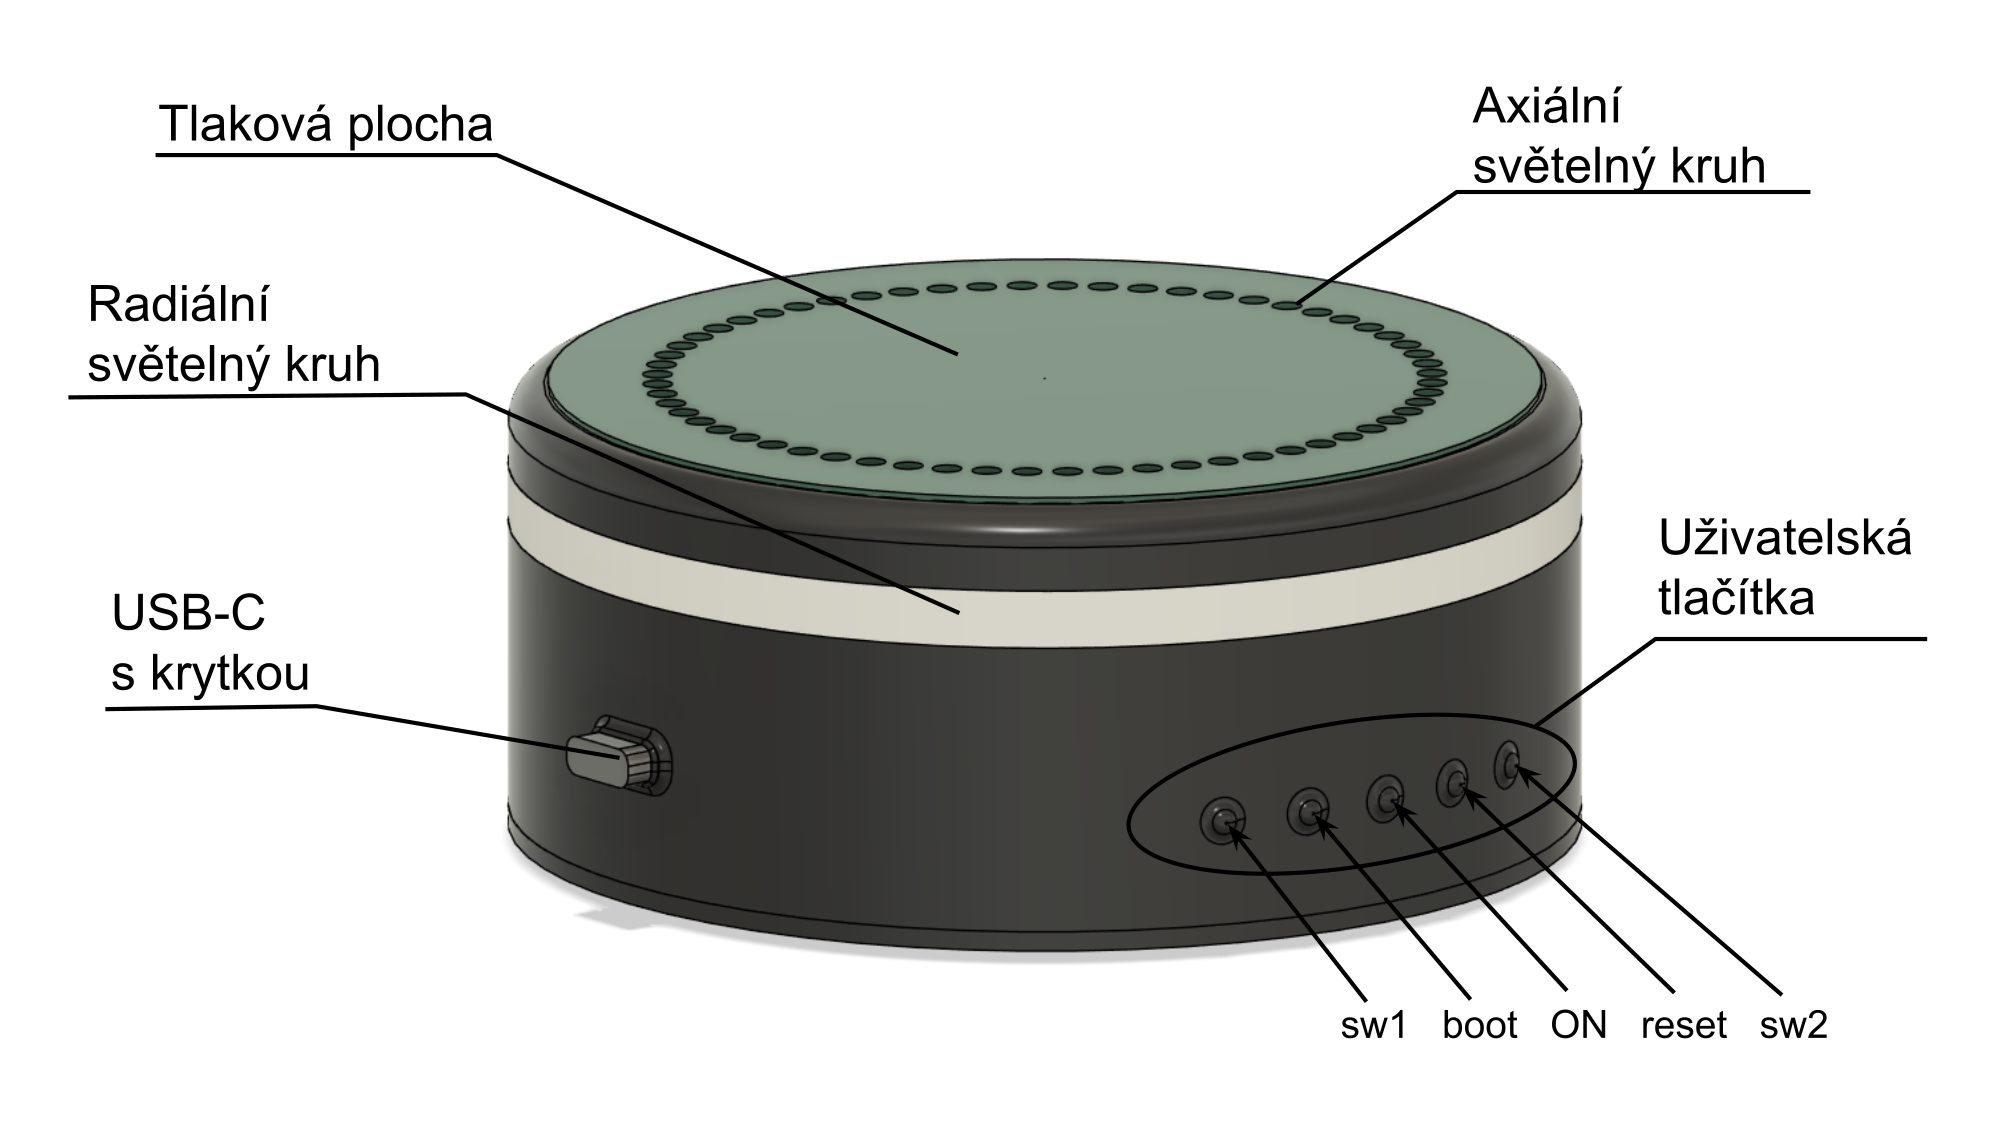
\includegraphics[width=\columnwidth]{text/PraktickaCast/img/AHS-nacrt.png}
	\end{textblock}
\end{frame} 

%%%%%%%%%%%%%
\begin{frame} 
	\frametitle{Výsledná konstrukce AHS}
	\centering
	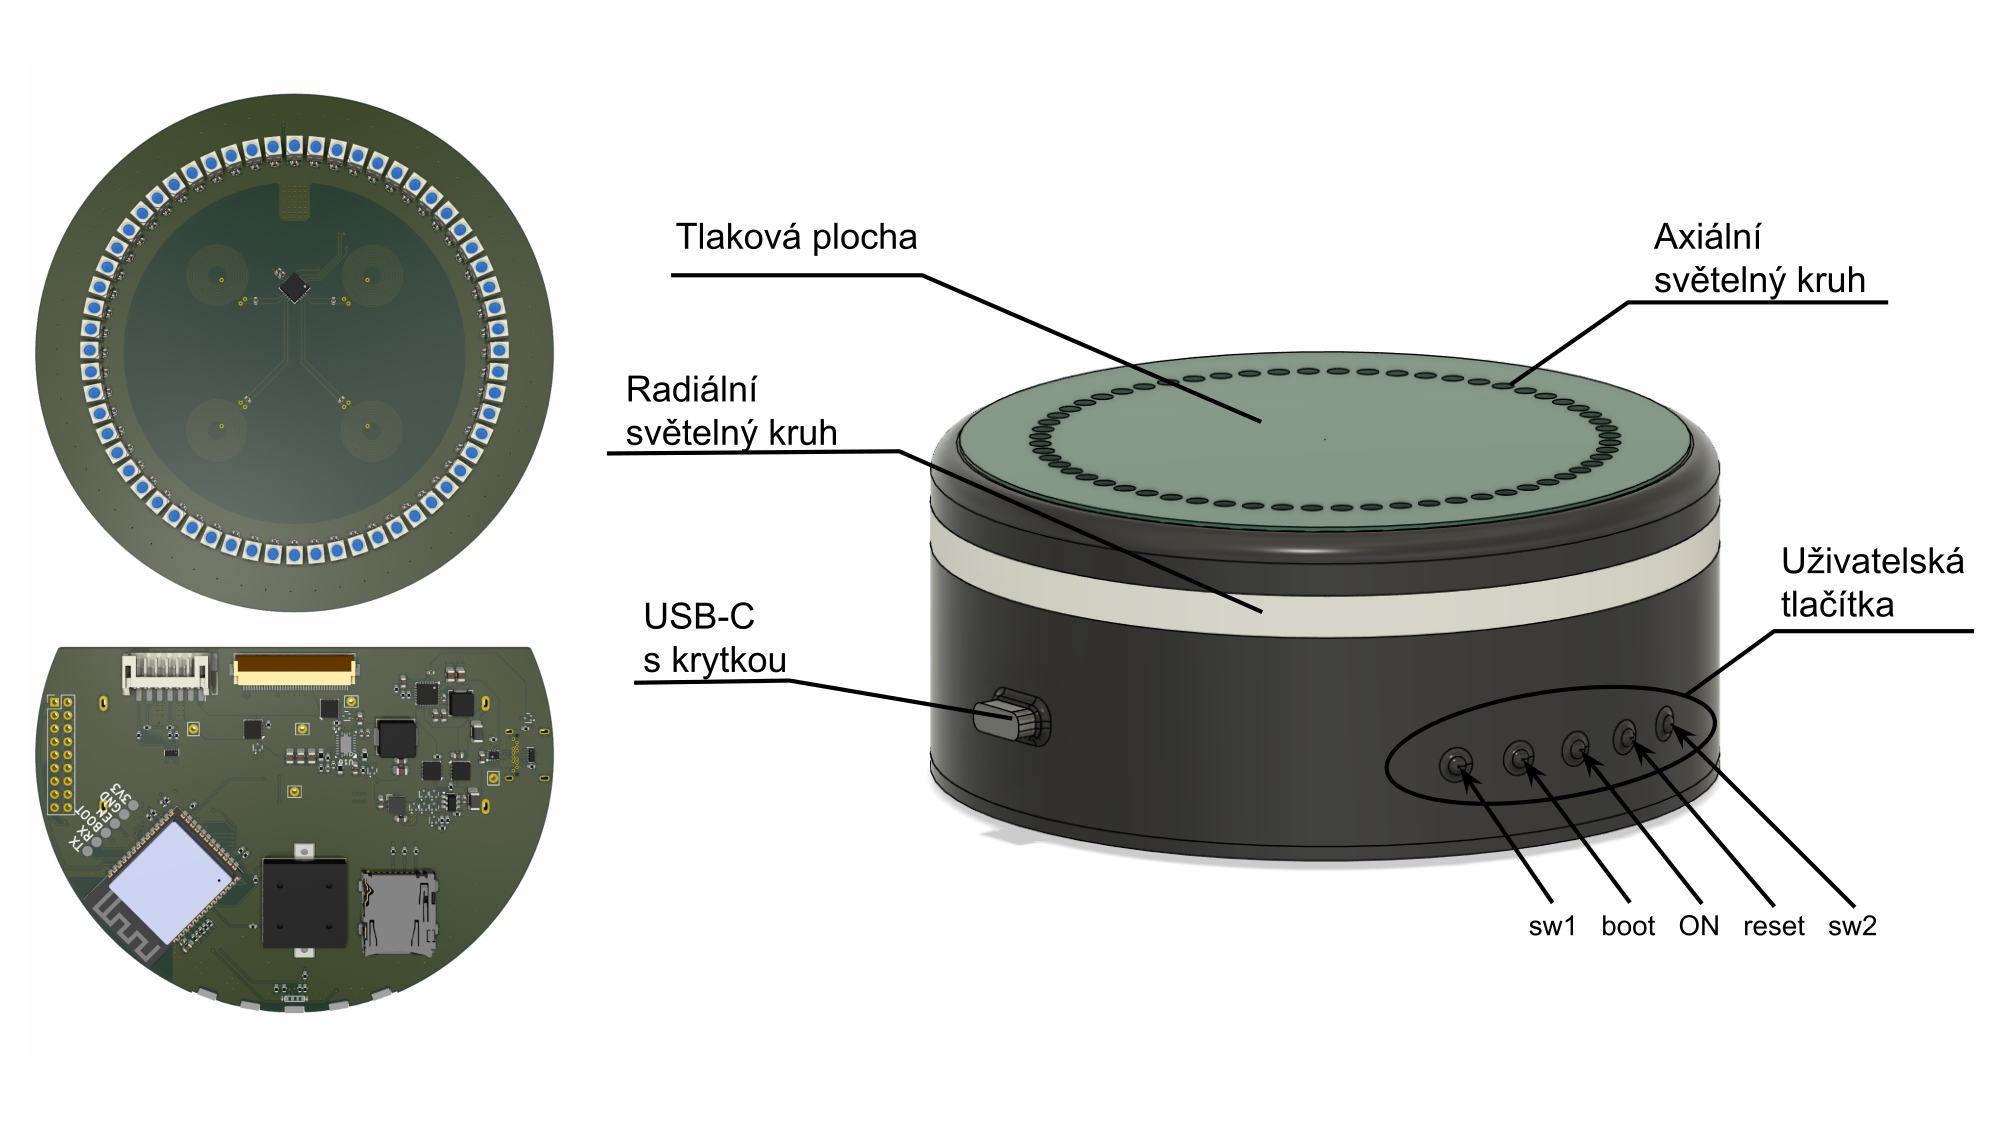
\includegraphics[width=\columnwidth]{text/PraktickaCast/img/AHS-kombo.png}
\end{frame} 

\begin{frame} 
	\frametitle{Tlaková plocha}
	\centering
	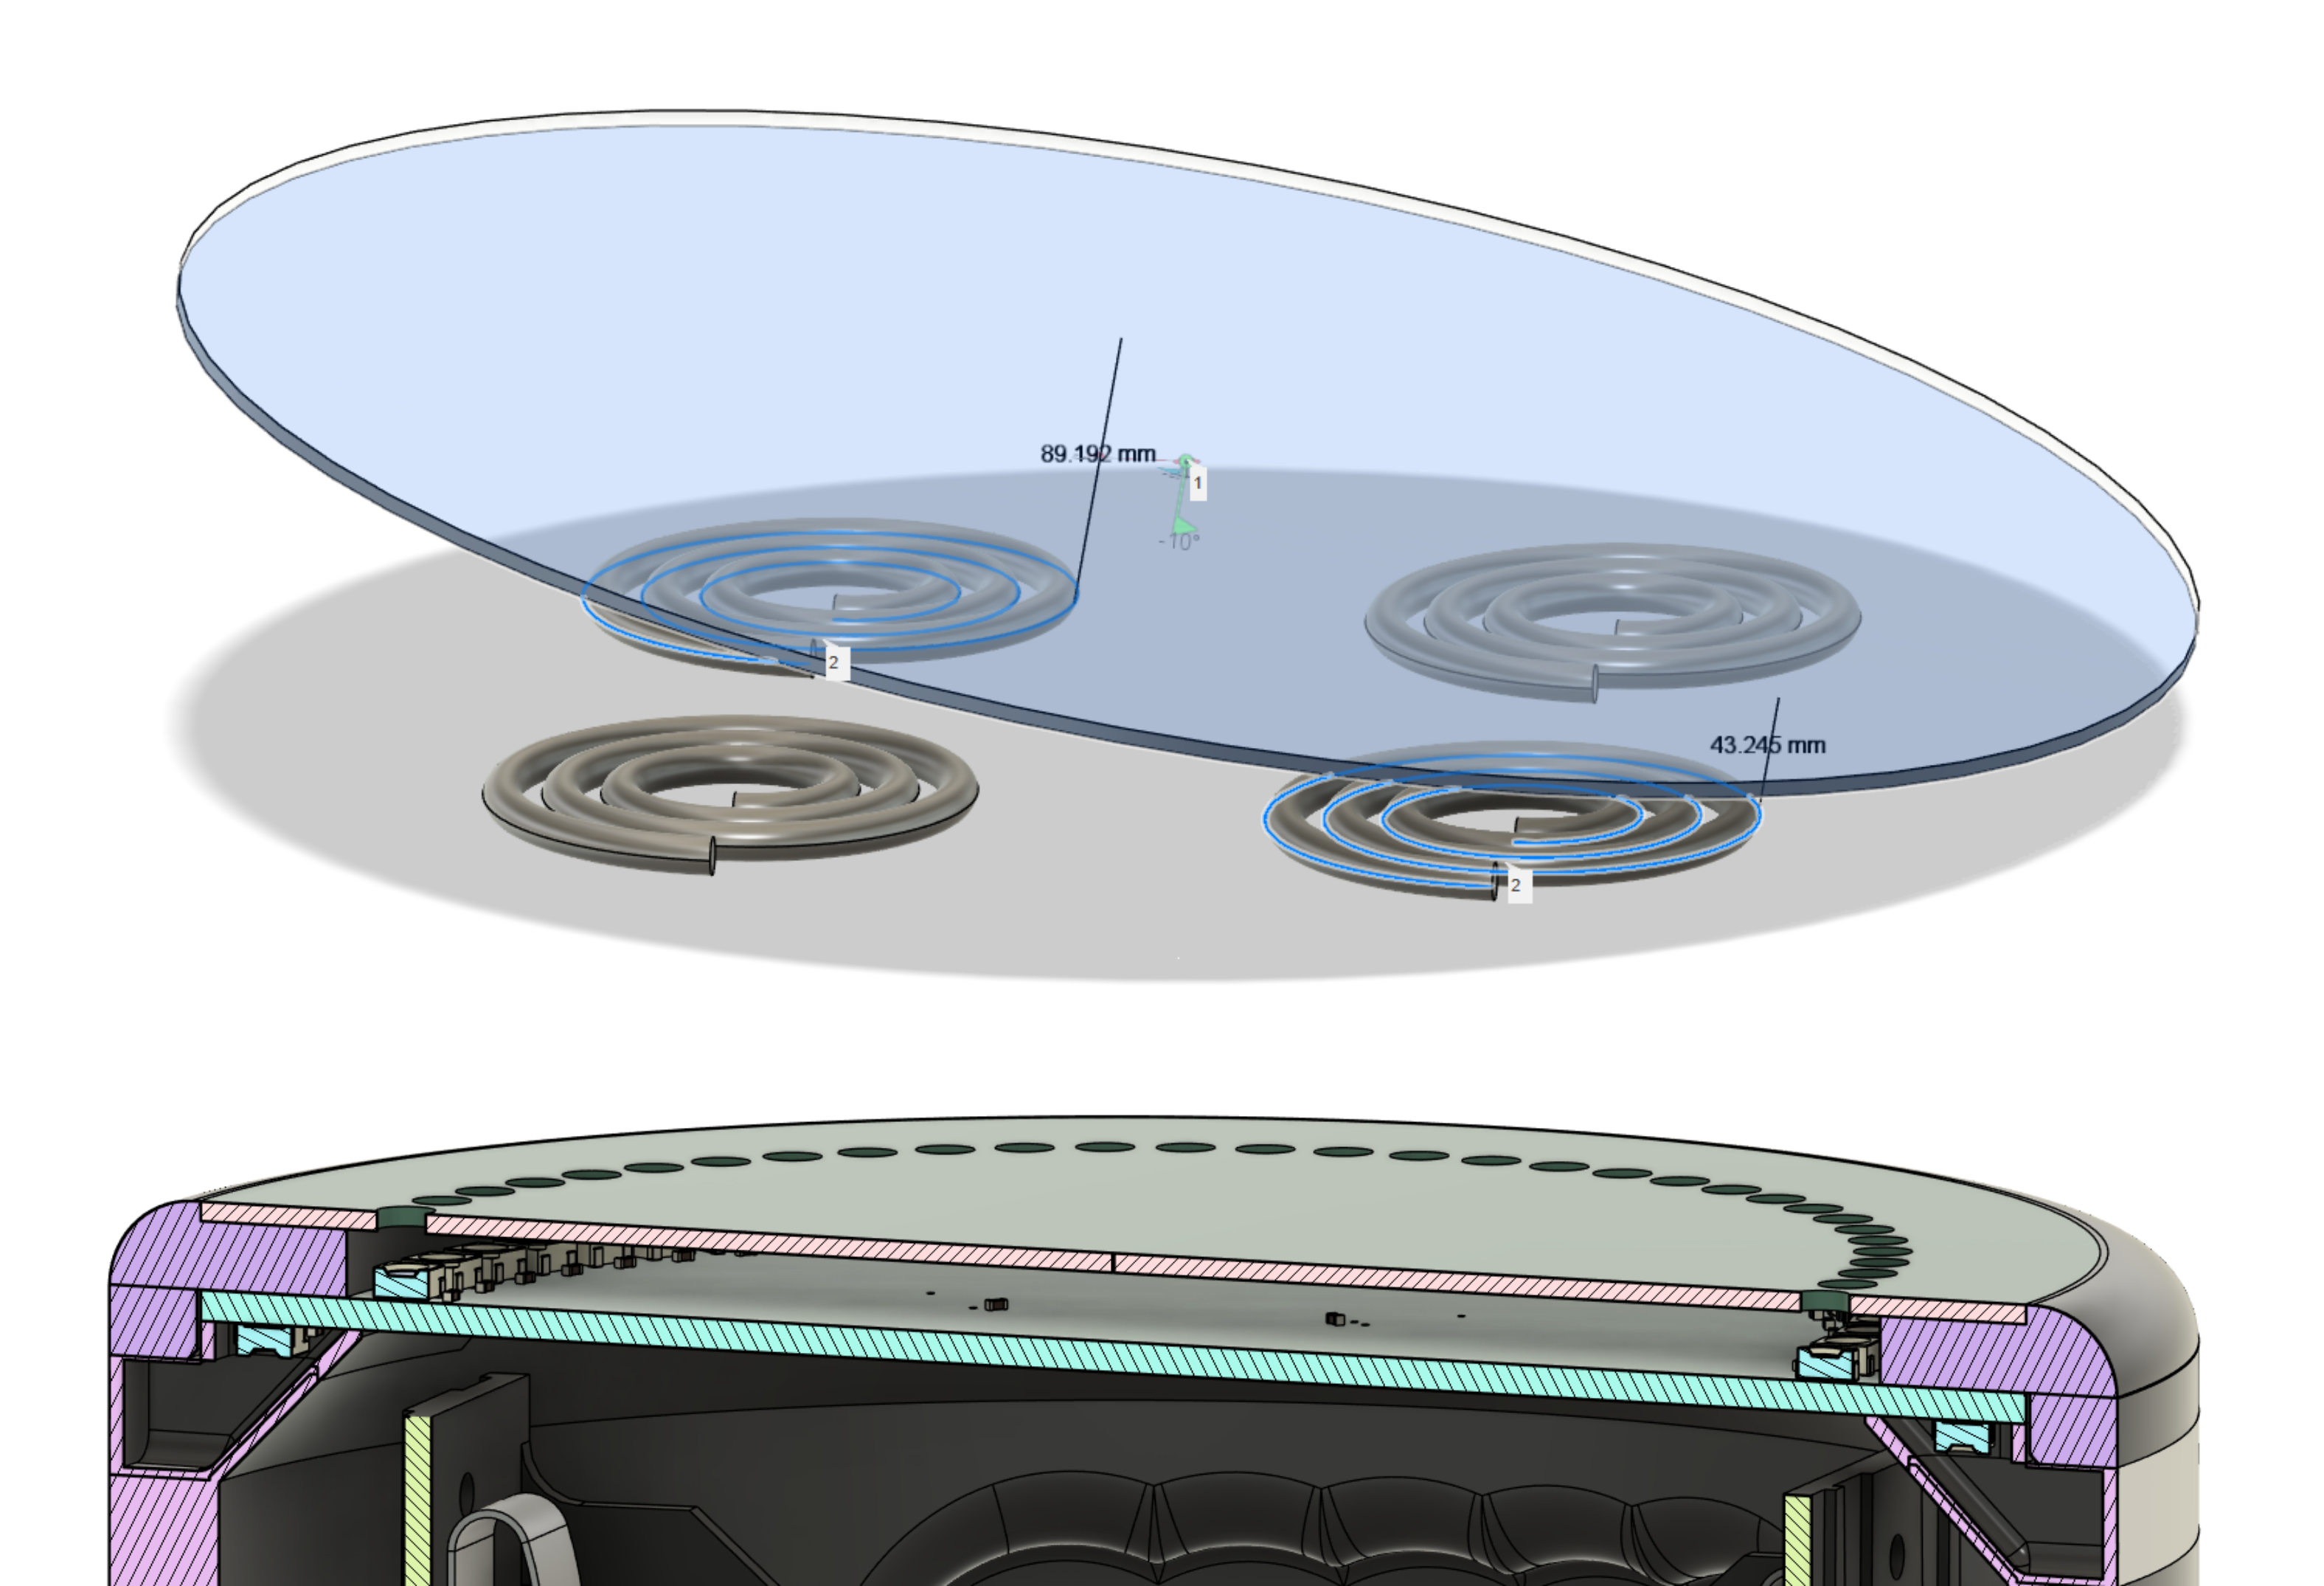
\includegraphics[width=0.8\columnwidth]{text/PraktickaCast/img/tlakovka-kombo.png}
\end{frame} 

%%%%%%%%%%%%%
\begin{frame} 
	\frametitle{Náčrt funkcí Semisemaforu}
	\vspace{10mm}
	\begin{itemize}
		\item Osobní zařízení
		\item Bezdrátová komunikace
		\item Zobrazení herních dat
		\item Jednoduchý uživatelský vstup
		\item Odolnost proti vodě
	\end{itemize}

	\begin{textblock}{8}(7.5,2.5)
		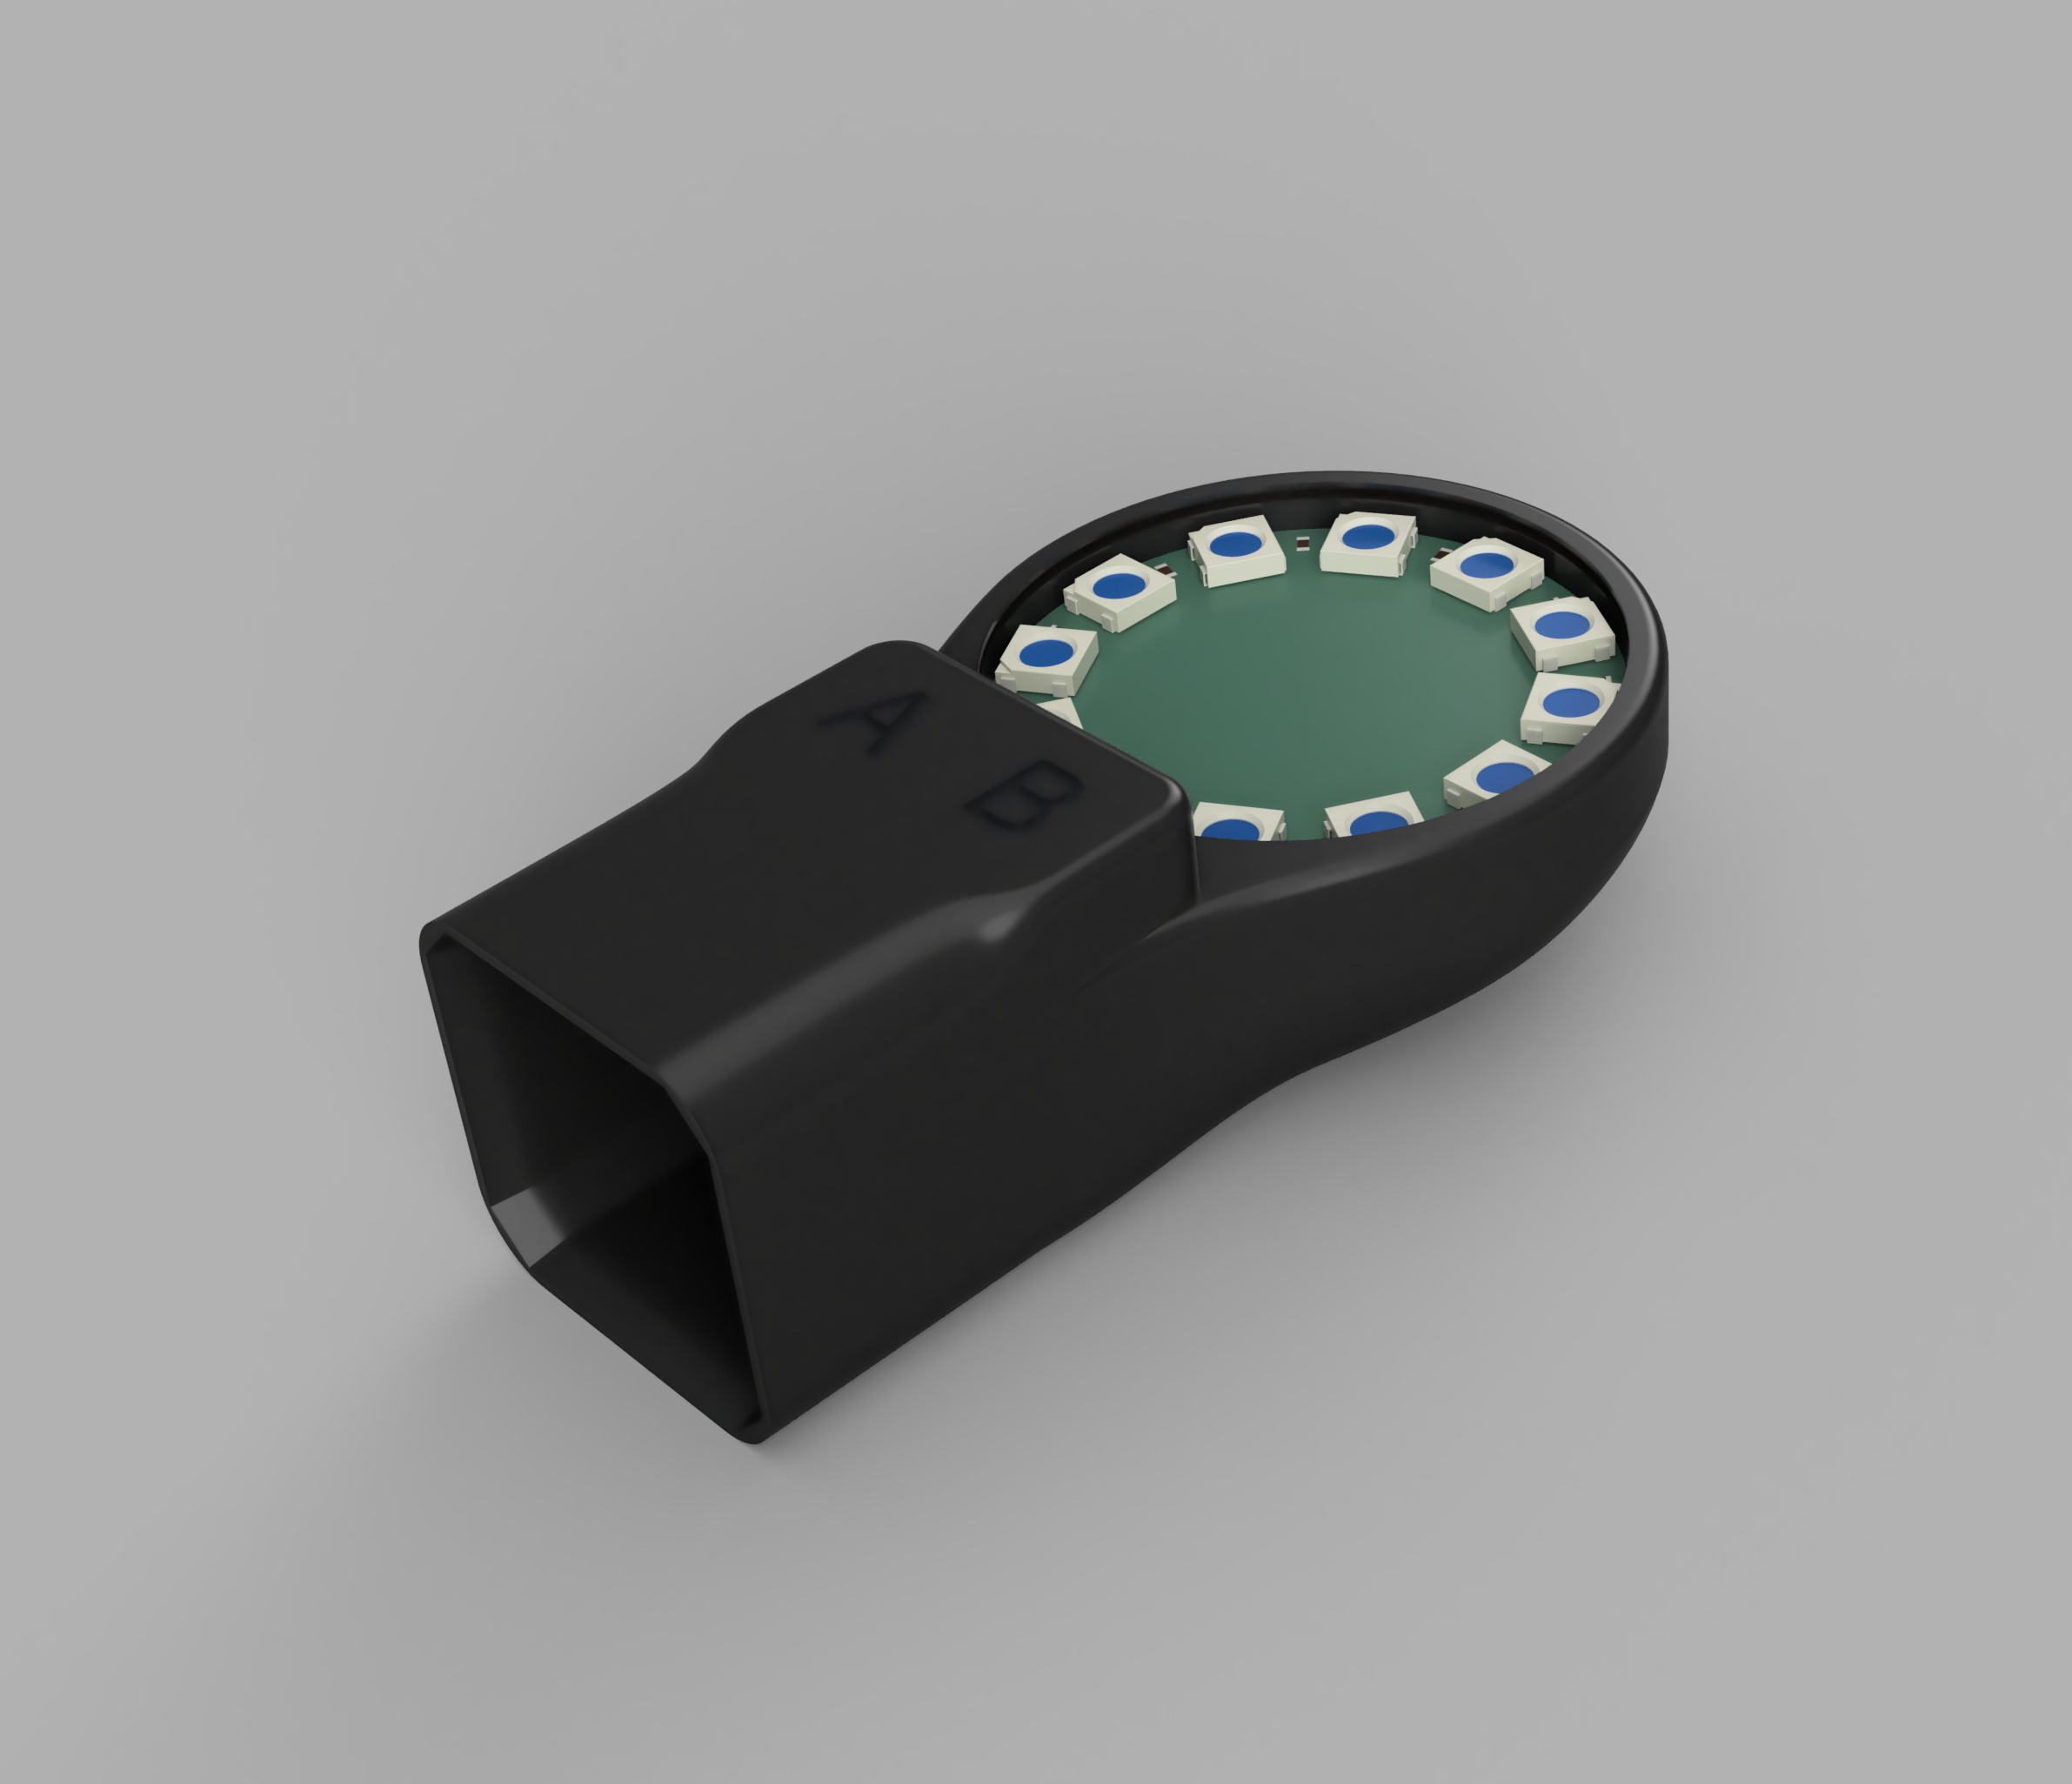
\includegraphics[width=\columnwidth]{text/PraktickaCast/img/SemiSemafor-BOX-render.png}
	\end{textblock}
\end{frame} 


% podekovani
\begin{frame}[c] 
% bez nadpisu snímku
	\frametitle{\mbox{ }}
	\begin{center}
		{\Huge Ukázka funkce}
		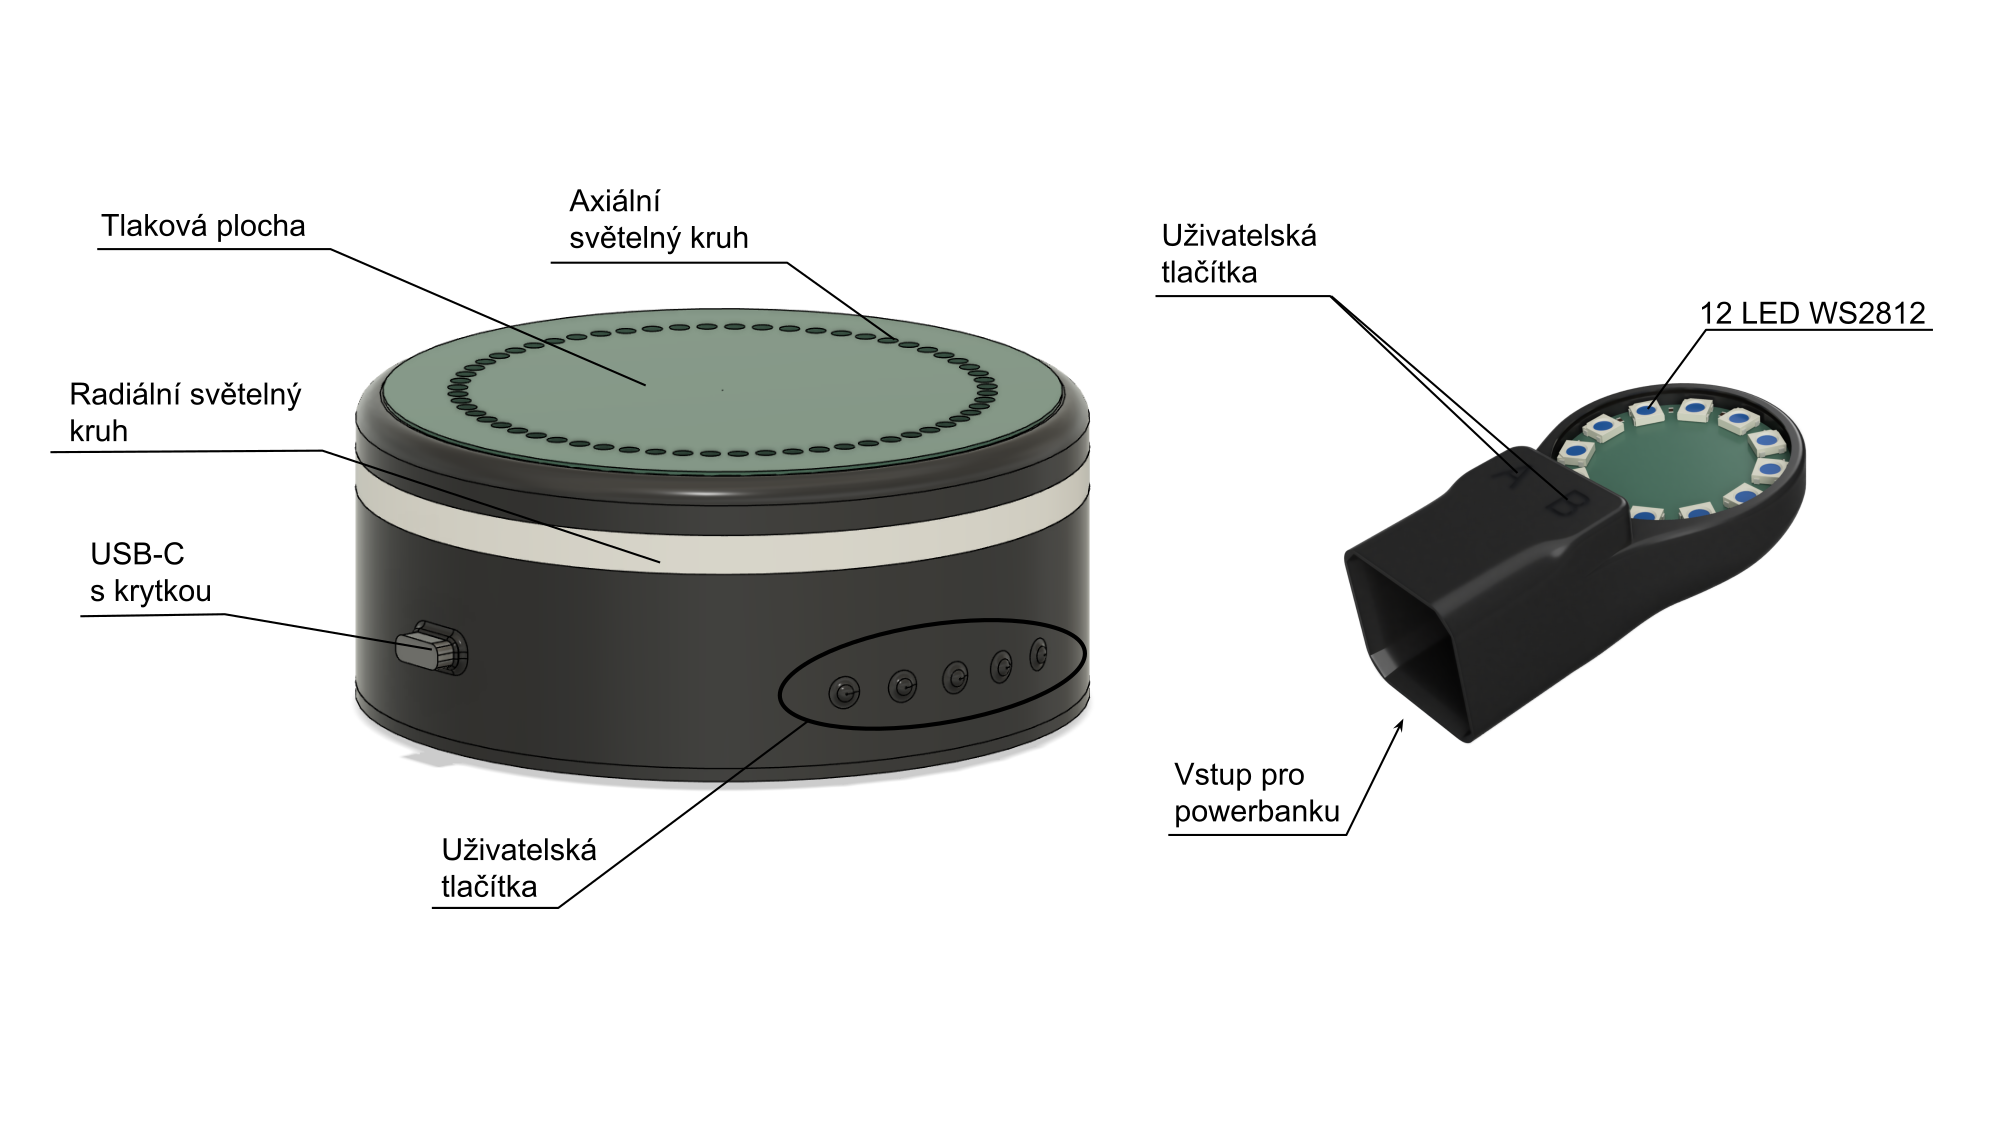
\includegraphics[width=\columnwidth]{text/PraktickaCast/img/AAHS-SS-kombo.png}
	\end{center}
\end{frame}




%%%%%%%%%%%%%
\begin{frame} 
	\frametitle{Jaký je váš odhad dokončení kompletní práce?}
	\vspace{10mm}
	\begin{itemize}
		\item Software AHS resp. Semisemaforu
		\item Moduly
		\item Webový portál pro nahrávání her
		\item Uživatelské programování pomocí bločku
	\end{itemize}
\end{frame}

%%%%%%%%%%%%%
\begin{frame} 
	\frametitle{Jaké jsou náklady spojené s výrobou vašeho zařízení? Předpokládám, že jej chcete komercionalizovat. Je to tak?}
	\vspace{5mm}
	\begin{itemize}
		\item Výrobní náklady na SemiSemafor
		\begin{itemize}
			\item DPS \(\approx\) 160 kč/ks \newline při výrobě 100ks
			\item Powerbanka \(\approx\) 110 kč/ks \newline při koupi 100ks
			\item 3D tisk \(\approx\) 20 kč/ks \newline při tisku 18ks současně
		\end{itemize}
		\item výsledná cena \(\approx\) 280 kč/ks \newline při výrobě 100ks
	\end{itemize}
	\begin{textblock}{6.5}(8.2,6)
		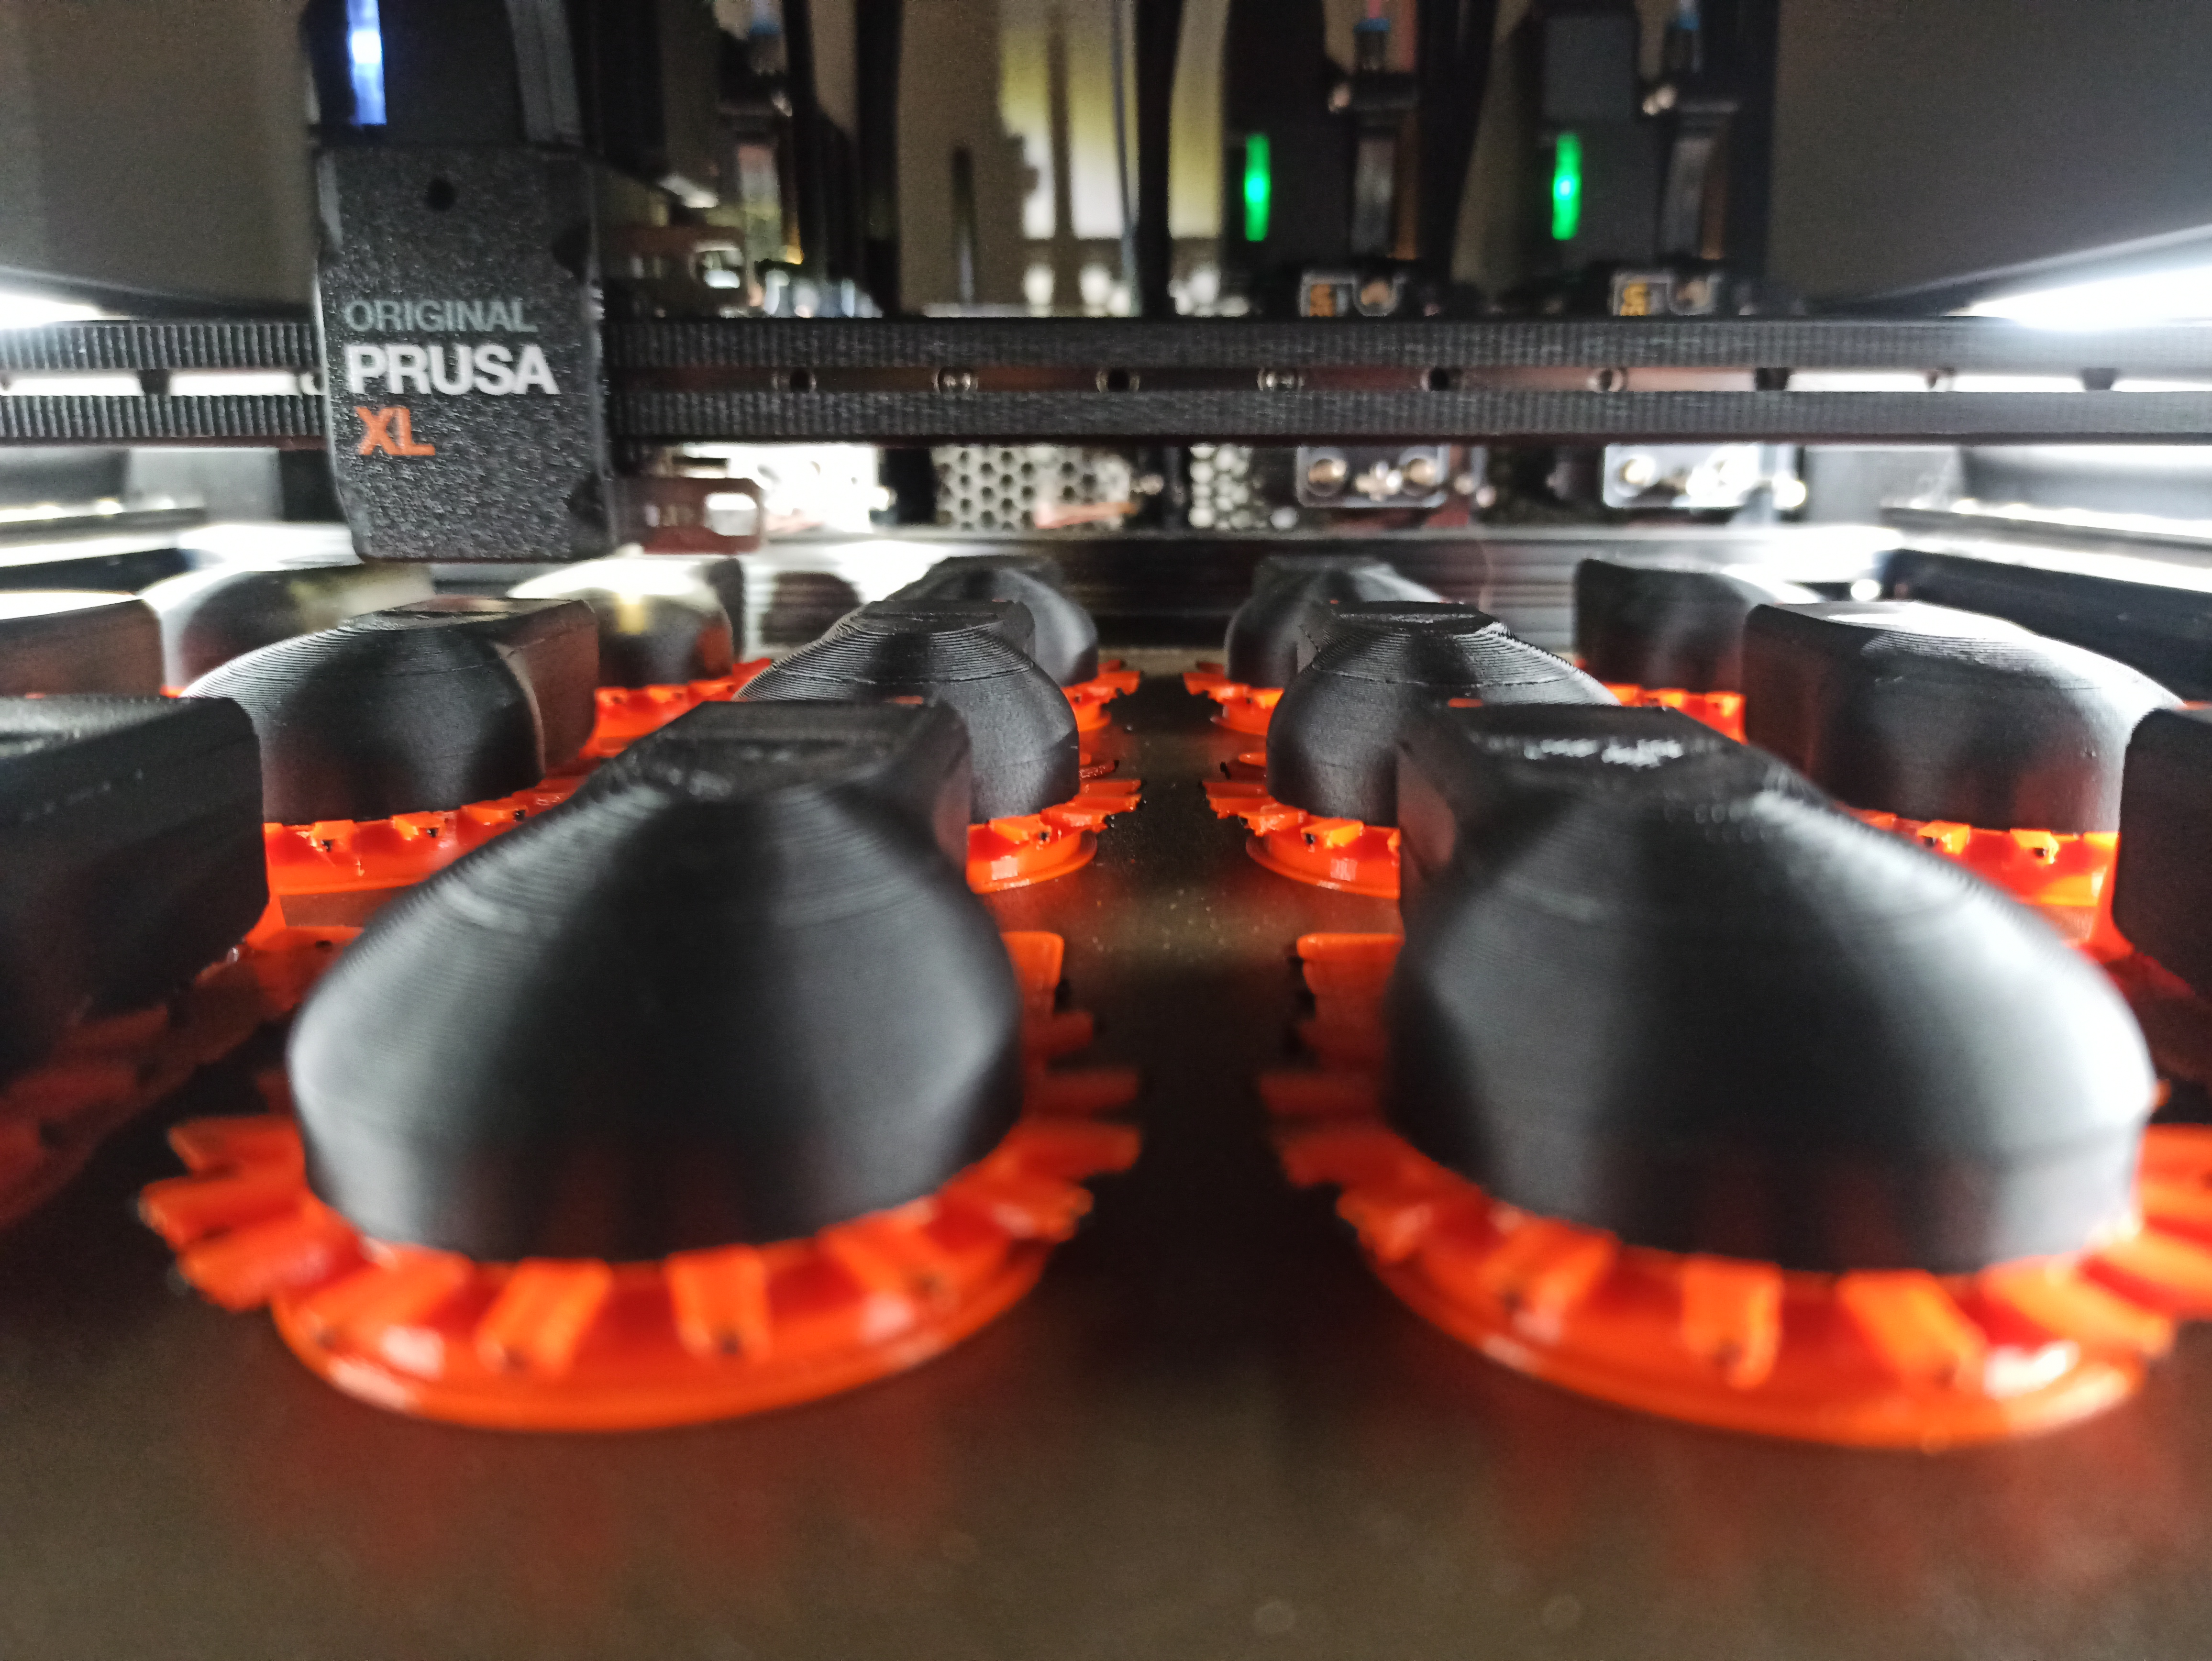
\includegraphics[width=\columnwidth]{text/PraktickaCast/img/SemiSemafor-tisk.jpg}
	\end{textblock}
\end{frame} 

\begin{frame} 
	\frametitle{Jaké jsou náklady spojené s výrobou vašeho zařízení? Předpokládám, že jej chcete komercionalizovat. Je to tak?}
	\hspace{-10mm}
	\begin{itemize}
		\item Výrobní náklady na AHS \newline(při výrobě 5ks):
		\begin{itemize}
			\item Hlavní deska \(\approx\) 1300 kč/ks
			\item LED deska \(\approx\) 680 kč/ks 
			\item Kontaktní plocha \(\approx\) 50 kč/ks 
			\item Baterie \(\approx\) 220 kč na zařízení 
			\item 3D tisk \(\approx\) 90 kč/ks
		\end{itemize}
		\item výsledná cena \(\approx\) 2260 kč/ks
	\end{itemize}
	\begin{textblock}{6.5}(8.5,5.5)
		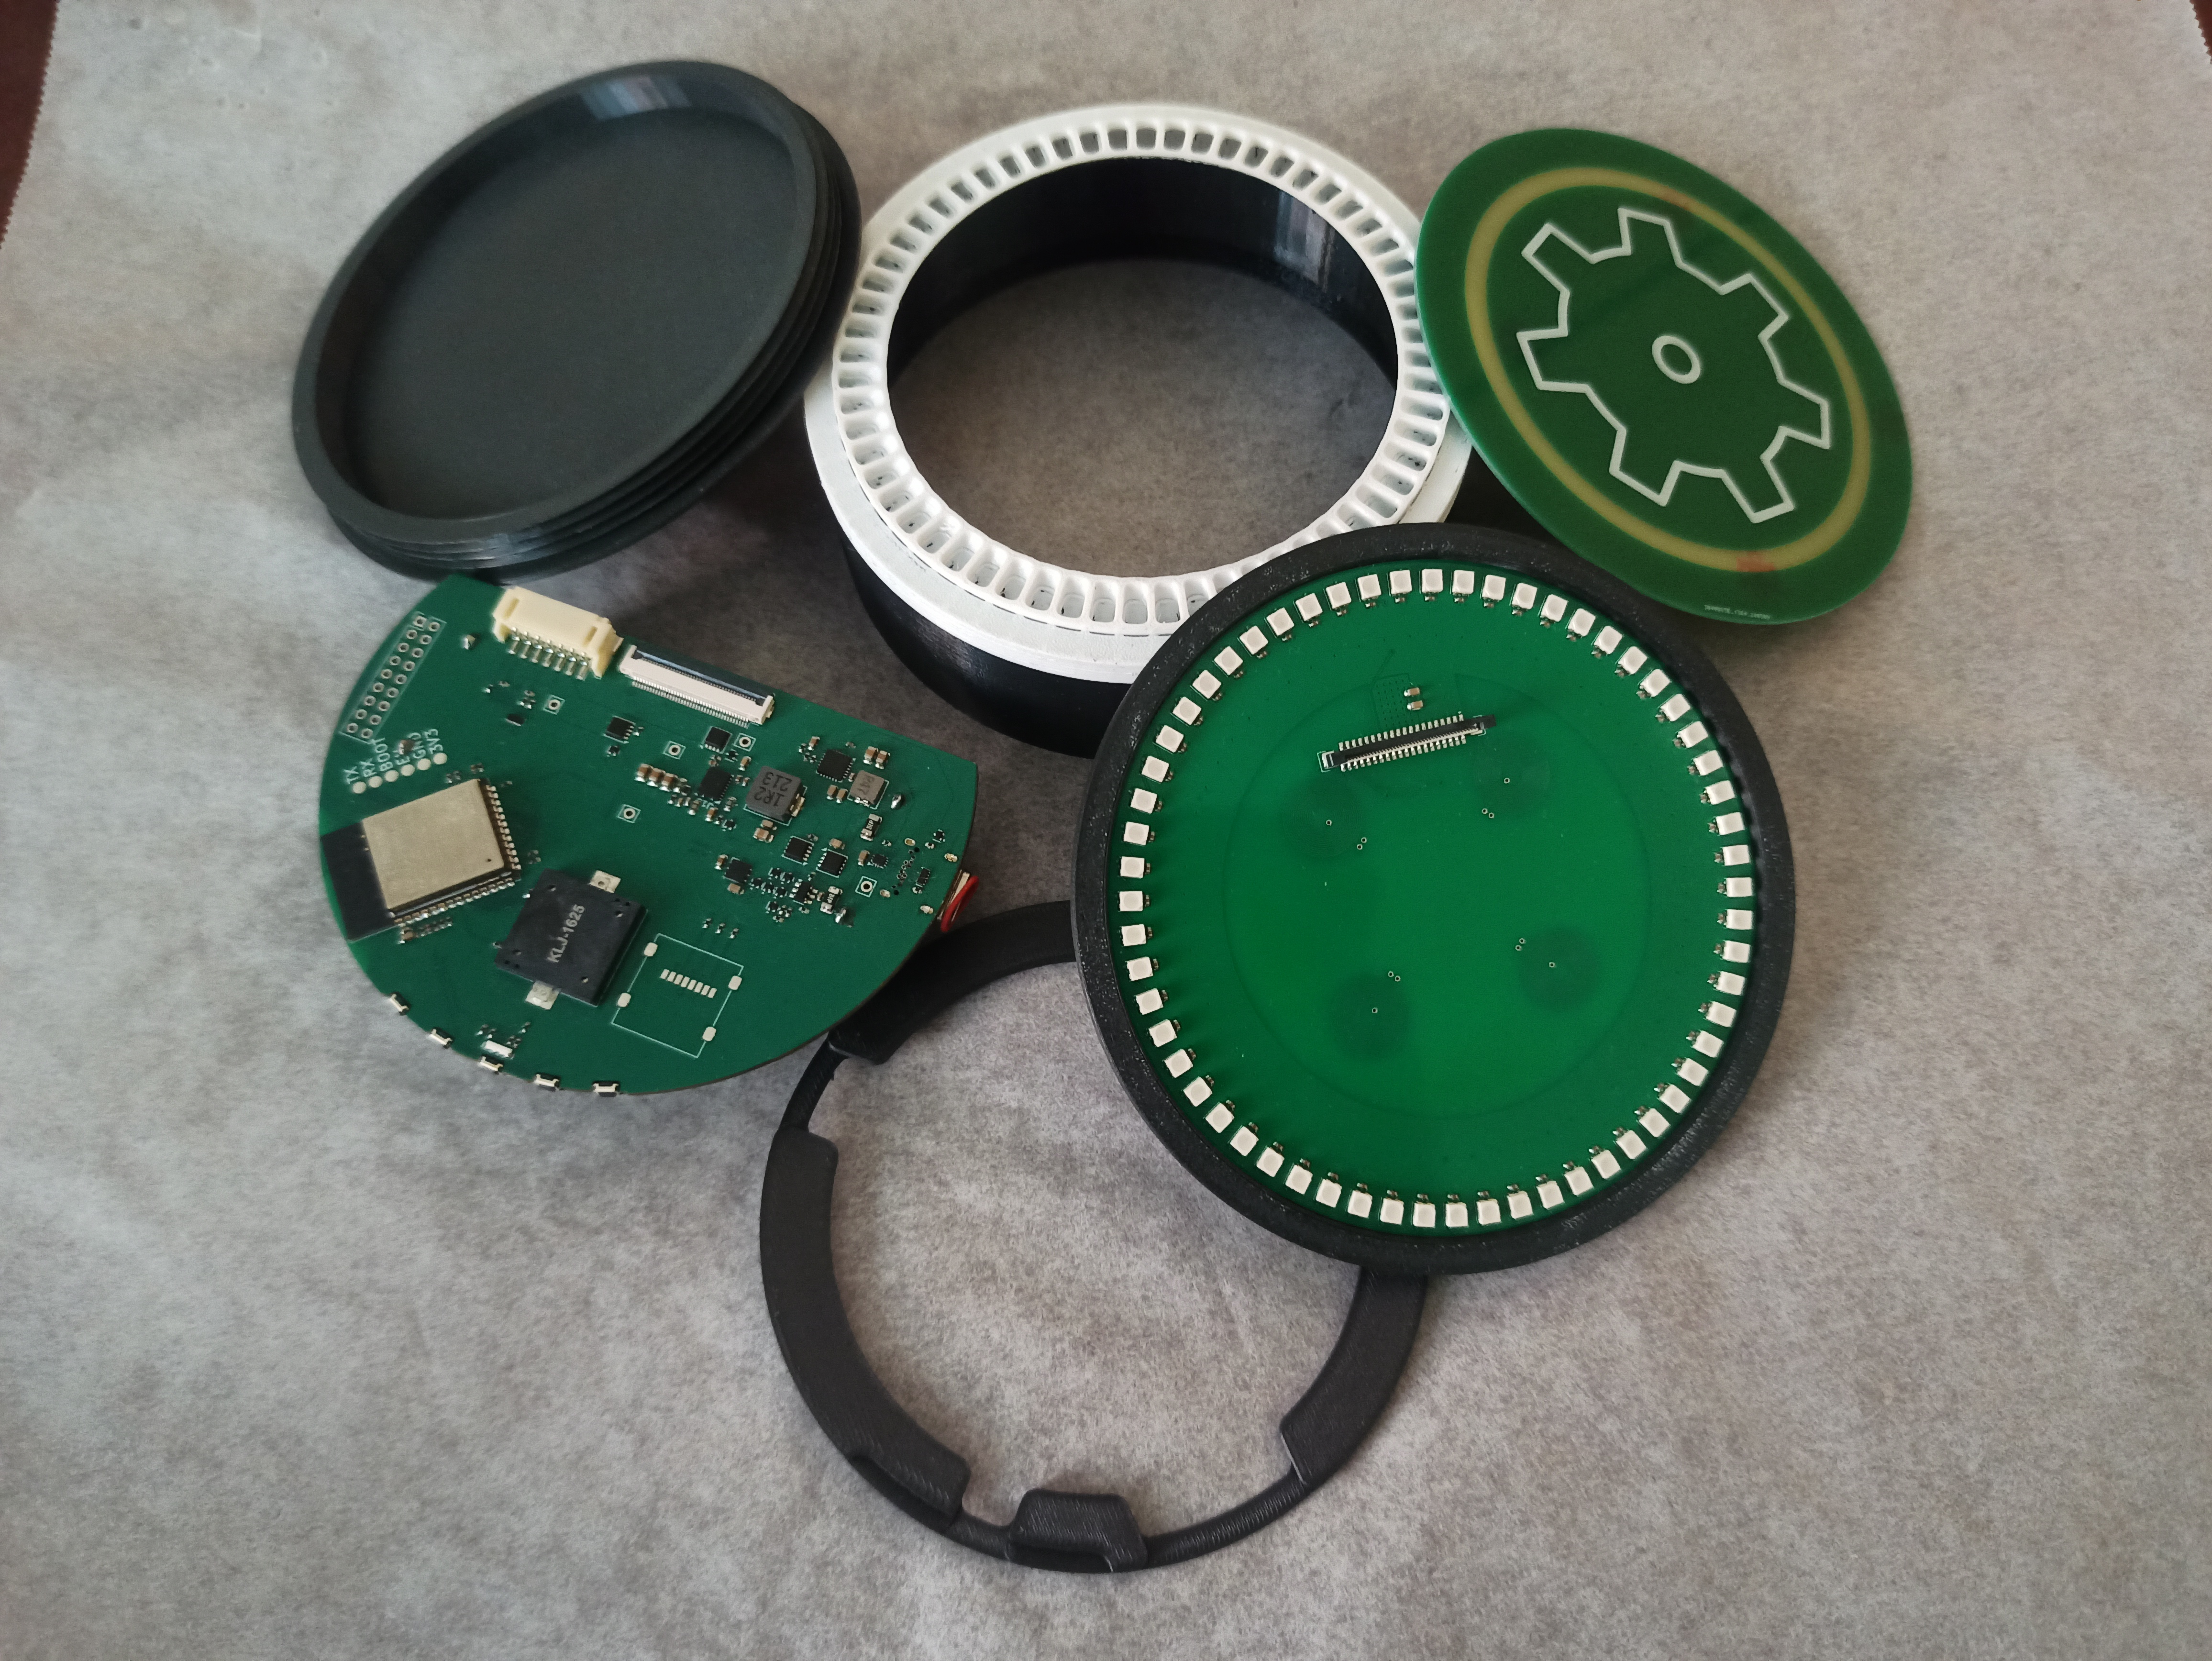
\includegraphics[width=\columnwidth]{text/PraktickaCast/img/AHS-rozsyp.jpg}
	\end{textblock}
\end{frame} 


%%%%%%%%%%%%%
% \begin{frame} 
% 	\frametitle{Závěr}
% 	\dots
% \end{frame}


% % podekovani
% \begin{frame}[c] 
% % bez nadpisu snímku
% 	\frametitle{\mbox{ }}
% 	\begin{center}
% 		{\Huge Děkuji za pozornost!}
% 	\end{center}
% \end{frame}

% otázky oponenta
	
\end{document}
